\chapter{Task-Priority Control}
\label{ch:tpc}
\label{chap:tpc}

This chapter explores various methods for task priority control, beginning with
an introduction to its fundamental concepts and a presentation of one of the
earliest and most straightforward techniques. It then continues into more advanced
approaches and concludes with a discussion of key implementation considerations,
including singularity robustness, for real-world robotic applications.

% -----------------------------------------------------------------------------
\section{Introduction}
\label{sec:tpc_intro}

Task priority control addresses the problem of managing multiple objectives simultaneously in a robotic system. It is a widely used methodology for handling redundancy in robots, enabling them to perform several tasks at once without compromising the executing of higher-priority objectives. Understanding the concept of tasks, their prioritization, and how multiple tasks interact is essential for understanding the fundamentals of task priority control.

A task refers to a specific objective or goal that a robotic system aims to achieve. Tasks can represent a wide variety of objectives, such as moving an end-effector to a desired position and orientation, maintaining a specific posture, avoiding joint limits, preventing collisions, or controlling specific velocities or accelerations at specific points. The tasks are typically described using functions, which map system states to task-specific outputs. These outputs are then often compared to desired values to determine the error and guide the control system towards achieving the task.

The prioritization of tasks is a key aspect of task-priority control. When a task is assigned a higher priority, it must be executed without being disturbed or compromised by lower-priority tasks. This means that the control system must balance the objectives of multiple tasks, ensuring that the higher-priority tasks are achieved while still allowing the lower-priority tasks to be executed. In practice, higher priority tasks are resolved first, and the remaining degrees of freedom are used to achieve the lower-priority tasks. For example, a robotic manipulator tasked with avoiding obstacles might prioritize obstacle avoidance over maintaining an exact end-effector position.

\sloppy{
In the following sections, we will develop the mathematical foundations of task-priority control, exploring the concepts of kinematic- and dynamic-level task-priority control.
}

% -----------------------------------------------------------------------------
\section{Kinematic-level Redundancy Resolution}

Kinematic-level redundancy resolution is a fundamental concept in task-priority control.
It is one of the first methods proposed for handling redundancy in a task-priority framework.
A fundamental assumption in kinematic-level redundancy resolution is that there
already exists a controller that can generate the desired generalized velocities \(\bm{\zeta}_d(t)\).
Considerations around this assumption will be discussed in later sections.
The mathematical concepts introduced in this section are presented in introductory
chapters in many of the articles and books on task-priority control, such as
\cite{hanafusa1981}, \cite{nakamura1987}, \cite{khatib1987}. An overview is
presented in \cite{chiaverini1997}.

\subsection{Velocity-level control}
\label{sec:velocity_level_control}

A task variable $\bm{\sigma}(t) \in \mathbb{R}^m$ is defined as a function of the robot's
state $\bm{\xi}(t) \in \mathbb{R}^n$:
\begin{align}
    \bm{\sigma}(t) = \bm{f}(\bm{\xi}(t)) \label{eq:def_task}.
\end{align}
A task can then be defined as the objective of keeping the task variable $\bm{\sigma}(t)$
close to a desired value $\bm{\sigma}_d(t) \in \mathbb{R}^m$. For instance, a task could
be the end-effector position of a robot manipulator or the orientation of a camera mounted
on a robot. By differentiating \autoref{eq:def_task} with respect to time, the task velocity
can be defined as
\begin{align}
    \dot{\bm{\sigma}}(t) = \frac{\partial \bm{f}(\bm{\xi}(t))}{\partial \bm{\xi}}
    \dot{\bm{\xi}}(t)= \left(\frac{\partial \bm{f}(\bm{\xi}(t))}{\partial \bm{\xi}}
    \bm{J}_{\Theta/q}(\bm{\xi}(t)) \right)\bm{\zeta}(t) \label{eq:def_task_jacobian},
\end{align}
where \(\bm{J}_{\Theta/q}\) describes the relation between \(\bm{\xi}\) and \(\bm{\zeta}\)
as shown in \autoref{eq:mod:jac}. It is important no note that this jacobian is dependent
on the parametrization choosen for the orientation; quaternion or Euler angles.
Collecting the parenthesis of \autoref{eq:def_task_jacobian} in a matrix
\(\bm{J}(\bm{\xi}(t))\), we get the following relation;
\begin{align}
    \dot{\bm{\sigma}}(t) = \bm{J}(\bm{\xi}(t))\bm{\zeta}(t).
\end{align}
The matrix \(\bm{J}(\bm{\xi}(t)) \in \mathbb{R}^{n \times m}\) is called the
\emph{task Jacobian}, or simply the \emph{Jacobian}, and maps the generalised
velocities $\bm{\zeta}(t)$ to the task velocity $\dot{\bm{\sigma}}(t)$.
The Jacobian is a function of the robot's state \(\bm{\xi}(t)\).
In the case where only one task is considered, one can use the pseudoinverse
to compute the minimum norm generalized velocities that will achieve the desired
task velocity. The generalized velocities are then given by
\begin{align}
    \bm{\zeta}_d(t) = \bm{J}^{+}(\bm{\xi}(t)) \dot{\bm{\sigma}}_d(t) \label{eq:task_priority}
\end{align}
where \(\bm{J}^{+}(\bm{\xi}(t))\) is the pseudoinverse of the Jacobian at the current
state \(\bm{\xi}(t)\). From now on the dependencies of $\bm{J}$, \(\bm{\xi}\)
and $\bm{\sigma}$ will be omitted for brevity.

In practice, the Jacobian might not represent the true kinematics of the robot.
Furthermore, depending on the task, the desired task velocity might not be feasible,
and there might be model errors and noise in the estimated generalized velocities making
the generalized velocities not equal to the desired generalized velocities. Because of this,
a feedback controller is needed to ensure that the desired task velocity is
achieved. Substituting the desired task velocity \(\dot{\bm{\sigma}}_d(t)\) in 
\autoref{eq:task_priority} with
a feedforward term and a feedback term, the generalized velocities can be computed as
\begin{align}
    \bm{\zeta}_d = \bm{J}^{+} \left(\dot{\bm{\sigma}}_d + \bm{\Lambda}\tilde{\bm{\sigma}}\right),
\end{align}
where $\tilde{\bm{\sigma}} = \bm{\sigma} - \bm{\sigma}_d$ is the error in the
task and the constant matrix $\bm{\Lambda}$ is a matrix that determines the
feedback gains.
Generalizing this to multiple tasks, we note that \autoref{eq:def_task_jacobian}
has a more general solution than \autoref{eq:task_priority} when $n > m$:
\begin{align}
    \bm{\zeta}_d = \bm{J}^{+} \dot{\bm{\sigma}}_d + (\mathbb{I} - \bm{J}^{+} \bm{J}) \bm{z},
\end{align}
for some arbitrary vector $\bm{z} \in \mathbb{R}^n$. The term
$(\mathbb{I}_n - \bm{J}^{+} \bm{J}) \bm{z}$ is recognized as the null space projection
of $\bm{z}$ onto the null space of the Jacobian matrix $\bm{J}$. By setting
$\bm{z}$ to some desired value, such as the generalized velocities of a lower-priority task,
one can achieve prioritization of tasks. To present the basic idea, consider the
tasks
\begin{subequations}
\begin{align}
    \bm{\sigma}_i &= \bm{f}_i(\bm{\xi}) \in \mathbb{R}^{m_i} &i &= 1, 2, \ldots, k \\
    \dot{\bm{\sigma}}_i &= \bm{J}_i(\bm{\xi}) \bm{\zeta} \in \mathbb{R}^{m_i} &i &= 1, 2, \ldots, k
\end{align}
\end{subequations}
with corresponding desired tasks
\begin{align}
    \dot{\bm{\sigma}}_{i,d}(t) \quad i = 1, 2, \ldots, k
\end{align}
Let $\bm{N}_i = \mathbb{I}_n - \bm{J}_i^{+} \bm{J}_i$ be the null space projection
matrix onto the null space of the Jacobian $\bm{J}_i$.
The desired generalized velocities are then given by
\begin{align}
    \bm{\zeta}_d = \sum_{i=1}^k \bm{N}_i^{\#}\bm{J}_i^{\#} \left(\dot{\bm{\sigma}}_{i,d} + \bm{\Lambda}_i \tilde{\bm{\sigma}}_i\right) \label{eq:task_priority_vel}
\end{align}
comparing this to the single task case, $\bm{N}_i^{\#}$ is the null space projection matrix
projecting a task onto the null space of all the higher-priority tasks.
\begin{align}
    \bm{N}_i^{\#} = \bm{N}_1 \bm{N}_2 \cdots \bm{N}_{i-1}
\end{align}
and the $\bm{J}_i^{\#}$ matrix is the projection matrix projecting a task onto the
subspace spanned by the task Jacobian.
\begin{align}
    \bm{J}_i^{\#} = \bm{J}_i^+
\end{align}
In general, several slightly different task priority control frameworks have
been proposed, following the same basic form as \autoref{eq:task_priority_vel}.
Although, slight variations in the form of the null space projection matrices
and the pseudoinverse matrices have been proposed. The methods include substituting
the pseudoinverse with the transpose of the Jacobian, and using augmented null space
projections.
The augmented null space projection is defined as
\begin{subequations}
    \label{eq:augmented_null_space}
\begin{align}
    \bm{N}_i^{\#} := \bm{N}_{1\cdots i-1} := \mathbb{I} - \bm{J}_{1\cdots i-1}^+ \bm{J}_{1\cdots i-1} \\
    \bm{J}_{1\cdots i-1} := \begin{bmatrix}
        J_1 \\
        J_2 \\
        \vdots \\
        J_{i-1}
    \end{bmatrix}
\end{align}
\end{subequations}
This gives rise to several different variants of the task priority control algorithm.
The variants discussed in \cite{antonelli2009} are summarized in the following table:
\begin{table}[h]
    \centering
    \begin{tabular}{|c|c|c|}
        \hline
        $J^{\#}$ & $N^{\#}$ & Algorithm's name \\
        \hline
        $\bm{J}^+$ & $\bm{N}_1 \bm{N}_2 \cdots \bm{N}_{i-1}$ & successive inverse-based projections \\
        $\bm{J}^+$ & $\bm{N}_{1\cdots i-1}$ & augmented inverse-based projections \\
        $\bm{J}^T$ & $\bm{N}_1 \bm{N}_2 \cdots \bm{N}_{i-1}$ & successive transpose-based projections \\
        $\bm{J}^T$ & $\bm{N}_{1\cdots i-1}$ & augmented transpose-based projections \\
        \hline
    \end{tabular}
    \label{tab:tpc_variants}
    \caption{Task priority control variants. Table from \cite{antonelli2009}}
\end{table}

Using the successive method, task velocities are progressively projected into the null space of higher-priority tasks by recursively multiplying null space projection matrices. In contrast, the augmented method constructs a single null space projection matrix by stacking the task Jacobians of all higher-priority tasks and then computing the pseudoinverse of this stacked matrix. This distinction is illustrated in \autoref{eq:augmented_null_space}.
It is important to emphasize that these two approaches are not equivalent. Null space projection matrices are generally not commutative, which means the successive method can yield a more conservative null space projection, whereas the augmented method often results in a less conservative projection, offering increased flexibility for lower-priority tasks.
From a computational perspective, the successive method is typically more efficient because it recursively computes the null space projection matrices. Conversely, the augmented method demands the computation of the pseudoinverse of a potentially large stacked Jacobian matrix, which is computationally more intensive.

% -----------------------------------------------------------------------------
\subsection{Acceleration-level control}

The previous chapter discusses the velocity-level control of tasks. It is also 
possible to determine the double derivative of the state variables corresponding to some
desired task acceleration. This is referred to as acceleration-level control.
To see this, consider \autoref{eq:def_task_jacobian} and differentiate
with respect to time once more:
\begin{align}
    \ddot{\bm{\sigma}} = \frac{d}{dt}\left(\bm{J} \bm{\zeta}\right) = \dot{\bm{J}} \bm{\zeta} + \bm{J} \dot{\bm{\zeta}}
    \label{eq:task_acc_jacobian}
\end{align}
Solving this equation for the derivative of the generalized velocities \(\dot{\bm{\zeta}}\) gives
\begin{align}
    \ddot{\bm{q}} = \bm{J}^{+} \left(\ddot{\bm{\sigma}} - \dot{\bm{J}}\dot{\bm{q}}\right) +
    \left(\mathbb{I} - \bm{J}^{+}\bm{J}\right) \bm{z} \label{eq:task_acc_control},
\end{align}
for some arbitrary vector $\bm{z} \in \mathbb{R}^n$. Inspired from the
velocity-level control, one can define the desired joint accelerations as
\begin{align}
    \ddot{\bm{q}}_d = \bm{J}^{+} \left(\ddot{\bm{\sigma}}_d
    - \dot{\bm{J}}\dot{\bm{q}}\right) \label{eq:task_priority_acc}.
\end{align}
One can impose the closed-loop characteristic of the task by defining the desired
task acceleration implicitly as
\begin{align}
    \left(\ddot{\bm{\sigma}}_d - \ddot{\bm{\sigma}}\right) +
    \bm{K}_d\left(\dot{\bm{\sigma}}_d - \dot{\bm{\sigma}}\right) +
    \bm{K}_p\left(\bm{\sigma}_d - \bm{\sigma}\right) = 0 \label{eq:task_acc}
\end{align}
where $\bm{K}_d$ and $\bm{K}_p$ are positive definite matrices. Substituting
\autoref{eq:task_acc} into the desired joint accelerations \autoref{eq:task_acc_jacobian},
and doing this for each task, one can get the desired joint accelerations:
\begin{subequations}
\begin{align}
    \bm{J}_i\ddot{\bm{q}} &= -\dot{\bm{J}}_i\dot{\bm{q}} + \ddot{\bm{\sigma}}_{i,d} 
    + \bm{K}_{d,i}\left(\dot{\bm{\sigma}}_{i,d} - \dot{\bm{\sigma}}_i\right)
    + \bm{K}_{p,i}\left(\bm{\sigma}_{i,d} - \bm{\sigma}_i\right) \\
    &=: \bm{h}_i(\bm{q}, \dot{\bm{q}}, t) \\
    \ddot{\bm{q}}_d &= \bm{J}_1^{+} \bm{h}_1 + \left(\mathbb{I} - \bm{J}_1^+\bm{J}_1\right) \bm{J}_2^{+} \bm{h}_2.
\end{align}
\end{subequations}
This method is called acceleration-level task priority control. The method can
be generalized to multiple tasks by using the same methods as presented in \autoref{sec:tpc_intro}.


\subsection{Low level control}

{
\color{red}
\begin{itemize}
    \item Add citations
    \item Decoupling of the quaternion vector in control
    \item Include chapter about set-based TPC
    \item Include chapter about how task-jacobians can be created.
\end{itemize}
}

The methods discussed above assume the existence of a controller capable of tracking the desired joint velocities \(\bm{\zeta}_d\). This implies that a lower-level controller must be designed and implemented, and its performance will directly affect the ability to follow the specified tasks.

A straightforward approach to tracking the desired generalized velocities is to use a simple \gls{pd} controller. However, because the robot’s state includes a unit quaternion and the generalized velocities are defined in the body frame—while the robot's state itself is defined in the \gls{ned} frame—some care must be taken during controller design. The controller can be written as:

\begin{subequations}
\label{eq:tau_pd}
\begin{align}
    \begin{bmatrix}
        \bm{p}_{nb,d}^n & {\bm{q}_{b,d}^n}^T & {\bm{\theta}_d}^T
    \end{bmatrix}^T
    &:=
    \bm{\xi}_{q,d}(t) := \int_{0}^{t} \bm{J}_q(\bm{q}_b^n(\tau))\bm{\zeta}_d(\tau)\,d\tau
    \\
    \begin{bmatrix} \eta_e & \bm{\varepsilon}_e^T\end{bmatrix}^T &:= \left(\bm{q}_{b,d}^n\right)^* \otimes \bm{q}_b^n
    \\
    \bm{\tau}_{PD} &= 
    \bm{K}_p \begin{bmatrix}
        \bm{R}_b^n(\bm{q}_b^n)^T\left(\bm{p}_{nb,d}^n - \bm{p}_{nb}^n\right) \\
        -\sgn{(\eta_e)} \bm{\varepsilon}_e \\
        \bm{\theta}_d - \bm{\theta}
    \end{bmatrix} + 
    \bm{K}_d  \left(\bm{\zeta}_d - \bm{\zeta} \right), 
\end{align}
\end{subequations}

where \(\bm{\tau} \in \R^{10}\) denotes the desired generalized forces on the body. The desired state \(\bm{\xi}_d\) is obtained by integrating the desired generalized velocities \(\bm{\zeta}_d\). The remaining symbols are defined in \autoref{sec:diff_kin}.

It's important to note that this controller does not account for low-frequency disturbances such as waves, ocean currents, or hydrodynamic forces. These will introduce low-frequency tracking errors. However, this limitation is mitigated by the higher-level, velocity-based task-priority controller, which includes feedback that adapts the desired velocity based on state error.

Minor improvements to the controller can still be made. While modeling the full dynamics of an \gls{aiauv} is challenging, gravity and buoyancy forces can be accurately captured if the vehicle’s mass and volume distributions are known. This leads to an extended controller, referred to as \gls{pd}+, which augments the original controller from \autoref{eq:tau_pd} with a compensation term:

\begin{align}
    \bm{\tau}_{PD+} = \bm{\tau}_{PD} + \bm{g}(\bm{\xi}(t)),
\end{align}

where \(\bm{g}(\bm{\xi}(t))\) is defined in \autoref{eq:modeling:g}. Provided the gravity and buoyancy forces are modeled correctly, this addition improves the steady-state tracking error, particularly in the vertical (downward) direction.

% -----------------------------------------------------------------------------
\section{Set-Based Task-Priority Control}

% -----------------------------------------------------------------------------
\section{Dynamic-level Redundancy Resolution}
\label{sec:tpc:dynamic_level}

Dynamic-level redundancy resolution solves the redundancy problem by considering
the robot's dynamics. This removes the need for a controller that can generate
the desired joint velocities $\dot{\bm{q}}_d(t)$, and instead uses the robot's
dynamic model to generate a generalized torque $\bm{\tau}_d(t)$ that will
be applied to the robot. There are several methods for dynamic-level redundancy
resolution, but here we will focus on the method presented in \cite{khatib2004}.
Consider the robot's dynamic model similar to models presented in previous sections:
\begin{subequations}
\begin{align}
    \bm{M}(\bm{q}) \ddot{\bm{q}} + \bm{N}(\bm{q}, \dot{\bm{q}}) \dot{\bm{q}} + \bm{g}(\bm{q}) &= \bm{\tau} \\
    \bm{q}, \dot{\bm{q}} ,\ddot{\bm{q}},\bm{\tau} &\in \mathbb{R}^n.
\end{align}
\end{subequations}
In the equation above, $N(\bm{q}, \dot{\bm{q}})$ represents the Coriolis and
damping forces acting on the robot. We consider a case with $2$ tasks, $\bm{\sigma}_t$
and $\bm{\sigma}_p$, and the corresponding Jacobians $\bm{J}_t$ and $\bm{J}_p$.
The essential equations concerning the tasks are:
\begin{subequations}
    \begin{align}
        \dot{\bm{\sigma}}_t &= \bm{J}_t(\bm{q}) \dot{\bm{q}} & \dot{\bm{\sigma}}_p &= \bm{J}_p(\bm{q}) \dot{\bm{q}} \\
        \ddot{\bm{\sigma}}_t &= \bm{J}_t(\bm{q}) \ddot{\bm{q}} + \dot{\bm{J}}_t(\bm{q}) \dot{\bm{q}} &
        \ddot{\bm{\sigma}}_p &= \bm{J}_p(\bm{q}) \ddot{\bm{q}} + \dot{\bm{J}}_p(\bm{q}) \dot{\bm{q}}.
    \end{align}
\end{subequations}
We define a dynamically consistent generalized inverse \cite{khatib1987} as
\begin{subequations}
    \begin{align}
        \bar{\cdot} &: \R^n \times \R^{m\times n} \rightarrow \R^{m\times n} & m &= 1, \cdots, n\\
        \bar{\cdot} &: (\bm{q},\bm{X}) \mapsto \bm{M}^{-1}(\bm{q})\bm{X}^T\left(
            \bm{X}\bm{M}^{-1}(\bm{q})\bm{X}^T.
        \right)^{-1}
    \end{align}
\end{subequations}
The dynamically consistent generalized inverse is used to project the system dynamics
onto the task space. For the sake of brevity, the dependencies of $\bm{q}$ and $\bm{\sigma}$
will be omitted in the following equations. We define the following properties and
select the applied generalized force $\bm{\tau}$ as
\begin{align}
    \bm{N}_t &:= \I - \bar{\bm{J}}_t \bm{J}_t &
    \bm{J}_{p|t} &:= \bm{J}_p \bm{N}_t &
    \bm{\tau} = \bm{J}_t^T \bm{f}_t + \bm{J}_{p|t}^T \bm{f}_p,
    \label{eq:force_application}
\end{align}
where $\bm{f}_t$ and $\bm{f}_p$ are forces applied in task space to be
specified. To build some intuition, consider the projected dynamics onto
the two task spaces, slightly abusing notation:
\begin{subequations}
    \label{eq:projected_dynamics}
\begin{align}
    \bar{\bm{J}}_t^T \left[
        \bm{M} \ddot{\bm{q}} + \bm{N} \dot{\bm{q}} + \bm{g} = \bm{\tau}
        \right]
    &\Rightarrow
    \bm{\Lambda}_t \ddot{\bm{\sigma}}_t + \bm{\mu}_t + \bm{p}_t = \bm{f}_t \\
    \bar{\bm{J}}_{p|t}^T \left[
        \bm{M} \ddot{\bm{q}} + \bm{N} \dot{\bm{q}} + \bm{g} = \bm{\tau}
        \right]
    &\Rightarrow
    \bm{\Lambda}_{p|t} \ddot{\bm{\sigma}}_p + \bm{\mu}_{p|t} + \bm{p}_{p|t} = \bm{f}_{p|t},
\end{align}
\end{subequations}
where
\begin{subequations}
\begin{align}
    \bm{\Lambda}_t &:= \left(\bm{J}_t \bm{M}^{-1} \bm{J}_t^T\right)^{-1} &
    \bm{\mu}_t &:= \bar{\bm{J}}_t^T \bm{N} \dot{\bm{q}} &
    \bm{p}_t &:= \bar{\bm{J}}_t^T \bm{g} \\
    \bm{\Lambda}_{p|t} &:= \left(\bm{J}_{p|t} \bm{M}^{-1} \bm{J}_{p|t}^T\right)^{-1} \label{eq:lambda_pIt} &
    \bm{\mu}_{p|t} &:= \bar{\bm{J}}_{p|t}^T \bm{N} \dot{\bm{q}} &
    \bm{p}_{p|t} &:= \bar{\bm{J}}_{p|t}^T \bm{g}
\end{align}
\end{subequations}
This is assuming that the Jacobians are full rank, implying that the task-space
mass matrices are invertible. From \autoref{eq:projected_dynamics}, it is clear
that one can use a feedback linearization technique to control the tasks. By
choosing the forces $\bm{f}_t$ and $\bm{f}_{p|t}$ as
\begin{subequations}
\begin{align}
    \bm{f}_t &= \bm{\Lambda}_t \bm{f}_t^* + \bm{\mu}_t + \bm{p}_t \\
    \bm{f}_{p|t} &= \bm{\Lambda}_{p|t} \left(\bm{f}_p^* - \ddot{\bm{\sigma}}_{\overline{p|t}}\right) + \bm{\mu}_{p|t} + \bm{p}_{p|t} \label{eq:osc_fp|t}\\
    \ddot{\bm{\sigma}}_{\overline{p|t}} &:= \ddot{\bm{\sigma}}_p - \ddot{\bm{\sigma}}_{p|t},
\end{align}
\end{subequations}
one can achieve the desired task accelerations $\bm{f}_t^*$ and
$\bm{f}_p^*$. The term $\bm{J}_t^T\bm{f}_t$ in \autoref{eq:force_application} can induce an acceleration in the 
controllable $p$-space, this is compensated for by the
$\ddot{\bm{\sigma}}_{\overline{p|t}}$ term \cite{sentis2004}:
\begin{align}
    \ddot{\bm{\sigma}}_{\overline{p|t}} = \bm{J}_p \bm{M}^{-1} \bm{J}_t^T \bm{f}_t
    + \bm{\Lambda}_{p|t}^{-1}\left(\bm{\mu}_{p|t} + \bm{p}_{p|t}\right)
    - \bm{\Lambda}_{p}^{-1}\left(\bm{\mu}_p + \bm{p}_p\right)
\end{align}
Assuming that the tasks are compatible, the desired task accelerations can be
shown to be
\begin{align}
    \ddot{\bm{\sigma}}_t &= \bm{f}_t^* & \ddot{\bm{\sigma}}_p &= \bm{f}_p^*.
\end{align}
In the case where $\bm{J}_{p|t}\bm{M}^{-1}\bm{J}_{p|t}^T$ in \autoref{eq:lambda_pIt}
is singular, the task-space mass matrix $\bm{\Lambda}_{p|t}$ can be generalized
as the Moore-Penrose pseudoinverse of the matrix \cite{khatib2004}:
\begin{align}
    \underline{\bm{\Lambda}}_{p|t} &:= \left(\bm{J}_{p|t} \bm{M}^{-1} \bm{J}_{p|t}^T\right)^{+} &
    \label{eq:lambda_pIt_pseudo}
\end{align}
Substituting $\bm{\Lambda}_{p|t}$ in \autoref{eq:osc_fp|t} with
$\underline{\bm{\Lambda}}_{p|t}$ in \autoref{eq:lambda_pIt_pseudo} allows for
accelerations in the non-conflicting directions in the $p$-space.

The method presented above has been generalized to multiple tasks in \cite{sentis2004}.
This will not be discussed in this thesis, but the essence of the method is the same
as presented above.

% -----------------------------------------------------------------------------
\section{Singularity Robustness}
\label{sec:tpc:sing_robust}

Considerations have to be taken into account when implementing the
pseudoinverse numerically on a computer. One of the most important considerations is the singularity
robustness of the algorithm. Although the pseudoinverse is defined for all matrices,
when the matrix is close to being singular, the pseudoinverse can be very sensitive
to small changes in the matrix. This might lead to very large input torques along
almost-singular directions. This problem is discussed extensively in \cite{chiaverini1997}.
The following section will discuss the singularity robustness of the algorithm used in this
thesis as proposed by \cite{chiaverini1997}.

First, consider the problem of taking the pseudoinverse of an arbitrary matrix $\bm{J}$.
As discussed in \autoref{sec:pseudoinverse}, the SVD of a matrix $\bm{J}$ can be
written as
\begin{align}
    \bm{J} = \bm{U} \bm{\Sigma} \bm{V}^T,
\end{align}
and the pseudoinverse of $J$ is
\begin{align}
    \bm{J}^+ = \bm{V} \bm{\Sigma}^+ \bm{U}^T.
\end{align}
Rewriting the $\bm{U}$ and $\bm{V}$ matrices as
\begin{subequations}
\begin{align}
    \bm{U} &= \begin{bmatrix} \bm{u}_1 & \bm{u}_2 & \cdots & \bm{u}_n \end{bmatrix} \\
    \bm{V} &= \begin{bmatrix} \bm{v}_1 & \bm{v}_2 & \cdots & \bm{v}_m \end{bmatrix}
\end{align}
\end{subequations}
where $\bm{u}_i$ and $\bm{v}_i$ are the columns of $\bm{U}$ and $\bm{V}$ respectively.
$\bm{J}$ and its pseudoinverse can be written as
\begin{subequations}
\begin{align}
    \bm{J} &= \sum_{i=1}^r \sigma_i \bm{u}_i \bm{v}_i^T \\
    \bm{J}^+ &= \sum_{i=1}^r \frac{1}{\sigma_i} \bm{v}_i \bm{u}_i^T.
\end{align}
\end{subequations}
From this, it is clear that when $\sigma_i$ is close to zero, the pseudoinverse
will be very sensitive to small changes in $\sigma_i$. One proposed solution to
this problem is the so-called \gls{dlsi} which is defined as
\begin{align}
    \bm{J}^* := \sum_{i=1}^r \frac{\sigma_i}{\sigma_i^2 + \lambda^2} \bm{v}_i \bm{u}_i^T.
\end{align}
We see that for large values of $\sigma_i$,
\begin{align}
    \frac{\sigma_i}{\sigma_i^2 + \lambda^2} \approx \frac{1}{\sigma_i},
\end{align}
and for small values of $\sigma_i$,
\begin{align}
    \frac{\sigma_i}{\sigma_i^2 + \lambda^2} \approx 0.
\end{align}
This will make the pseudoinverse well-conditioned for all values of $\sigma_i$.
The trade-off is that the \gls{dlsi} will not be the true pseudoinverse.
This might lead to tasks with lower priority affecting the higher-priority tasks and
breaking some of the assumptions made when proving stability and task consistency.

A way to make the pseudoinverse more accurate when far from singularities is to
use the \gls{vdlsi} proposed by \cite{chiaverini1997}.
This uses the fact that there is no need to damp the pseudoinverse when far from singularities.
The gls{vdlsi} is defined as
\begin{subequations}
\begin{align}
    \bm{J}^{\circ} := \sum_{i=1}^r \frac{\sigma_i}{\sigma_i^2 + \lambda_i^2(\sigma_i)} \bm{v}_i \bm{u}_i^T \\
    \lambda_i^2(\sigma_i) = \begin{cases}
        0 & ,\sigma_i \geq \varepsilon \\
        \left(1-\left(\frac{\sigma_i}{\varepsilon}\right)^2\right)\lambda_{max}^2 & ,\sigma_i < \varepsilon,
    \end{cases}
\end{align}
\end{subequations}
where $\lambda_{max}^2$ and $\varepsilon$ are parameters that can be tuned. $\lambda_{max}$
determines the maximum damping factor and $\varepsilon$ determines a threshold for when
to start damping the pseudoinverse based on how close the singular values are to zero.
To better illustrate the difference between the different methods, see \autoref{fig:1_x}
showing the \gls{lsi}, \gls{dlsi} and \gls{vdlsi} on a scalar matrix for $\lambda=\epsilon=0.1$.

\begin{figure}[h]
    \centering
    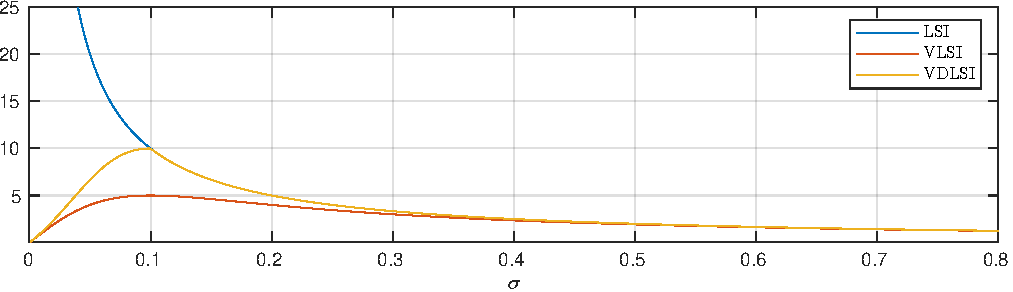
\includegraphics[width=\textwidth]{assets/singval.pdf}
    \caption{Comparison of the \gls{lsi}, gls{dlsi} and gls{vdlsi} on a scalar matrix.}
    \label{fig:1_x}
\end{figure}



